\chapter{Instrumental variabels methods}
本章笔记均为书面形式,只汇总概要,具体内容看书面笔记.

这一章主要讲述了一种估计causal effect的新思路. 

在第三章和第四章中,估计causal effect的重要假设就是ignorability assumption,给定covariates X,treatment与potential outcome独立. 控制这些covariates足够控制所有的confounding.

然而当存在unmeasured confounding时, match和iptw的方法得到的估计量是有偏差的,这种偏差称为hidden bias,是一种潜在的偏差. 本章讲述的instrumental variable methods可以在存在unmeasured confounding的情况下,很好地解决causal effect的估计问题. 只不过此时我们不再是估计average causal effect,而是local average causal effect,针对的估计对象从whole population变成了subpopulation(Compliers).

\section{Introduction to instrumental variables}
\subsection{Two types of causal graphics}
\subsection{The meaning and characters of Z}


\section{Randomized trials with noncompliance}
\subsection{Regard Z as treatment assignment}
\begin{itemize}
	\item The difference between assigned treatment and treatment received.
\end{itemize}
\subsection{Noncompliance}
\subsection{Potential treatment}
\subsection{Causal effect of Z on A}
\subsection{Causal effect of Z on Y}
\subsection{Causal effect of A on Y}


\section{Compliance classes}
\subsection{Four classes of subpopulation}
\begin{itemize}
	\item Principle stratification according to potential treatment$A^0,A^1$.
\end{itemize}

\subsection{Local average treatment effect}
\begin{itemize}
	\item Population causal effect and local causal effect.
\end{itemize}

\subsection{Four classes in Observational data}

\section{Assumptions}
\subsection{Assumptions about IVs}
\subsection{Assumptions about identification of causal effect}

\section{Causal effect identification and estimation}
\begin{itemize}
	\item Intention to treat effect(ITT).  We can identify ITT. 因为Z是randomized的,所以potential outcome的分布与Y的条件分布存在一一对应关系. 
	\begin{equation}
	ITT=E(Y^{Z=1}-Y^{Z=0})=E(Y|Z=1)-E(Y|Z=0).
	\end{equation} 
	\item 注意如何从ITT推导出Complier average causal effect.
	\item Compliers所占的比重推导. P(Compliers)=E(A$|$Z=1)-E(A$|$Z=0).
	\item CACT $>=$ ITT. 分析原因.
\end{itemize}

\section{IVs in observational data}
\subsection{Identifying an IV}
使用IV的挑战在于:如何寻找一个有效的工具变量,使之只影响treatment,而不影响outcome.

在这一节中举例说明了什么样的变量可以作为工具变量,并给出了三个常用的工具变量实例:
\begin{itemize}
	\item Mendelian randomization assumption: genetic variant.
	\item Provider preference(分配treatment的人的偏好).
	\item Quarter of birth.
\end{itemize}

\section{Two-stage regression}
\subsection{Recall: Ordinary least square}
对于估计causal effect的回归模型\ref{ceols}来说,最小二乘失效的原因是什么?
\begin{equation}
\label{ceols}
Y=\beta_0 + A\beta_1 + \epsilon
\end{equation}

\r{误差项与回归变量有关.} 此时A在计量经济学中称为内生变量.

\subsection{Stage 1:Regress treatment received A on the instrumental variable Z}
\subsection{Stage 2:Regress the outcome Y on the fitted value $\hat{A}$ from stage 1}

\subsection{Implement}
\begin{itemize}
	\item The interpretation of $\beta_1$.
	
\end{itemize}
%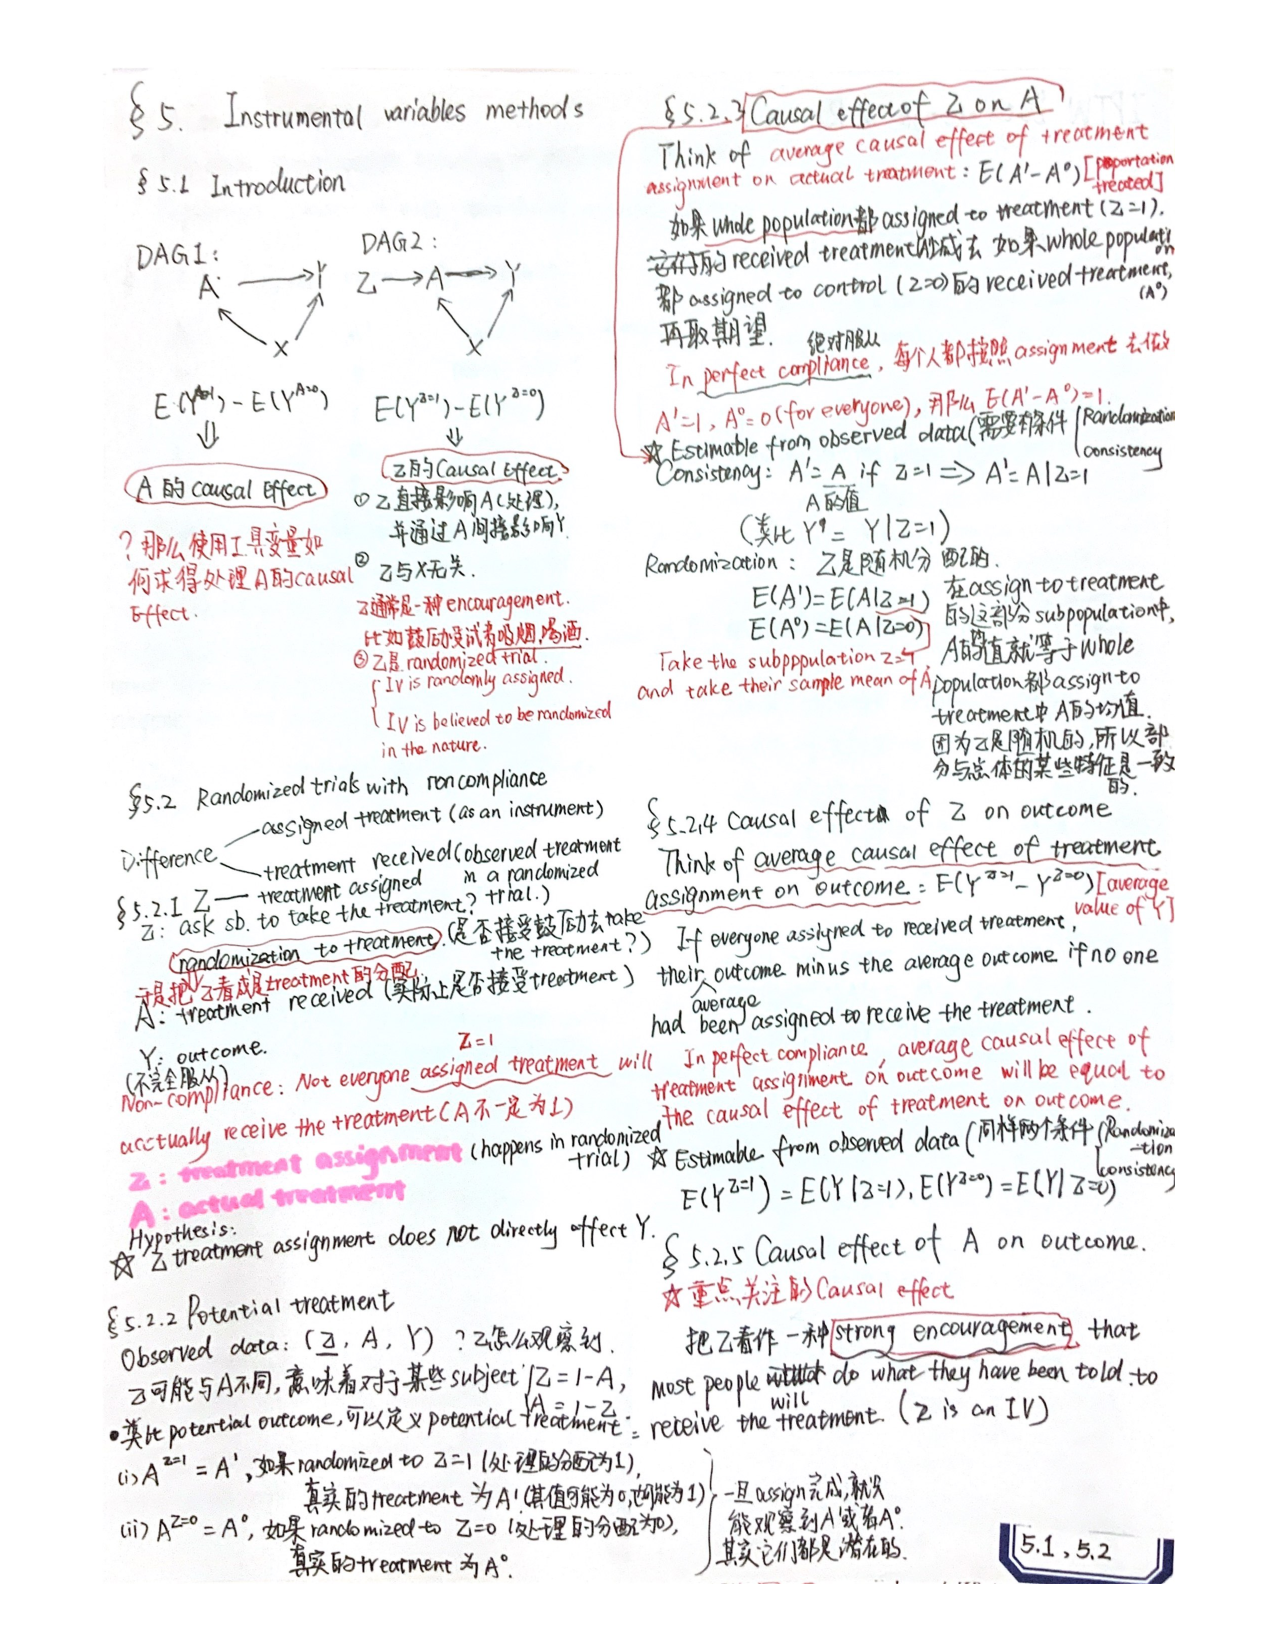
\includepdf[pages=-]{figure/5p1.pdf}
%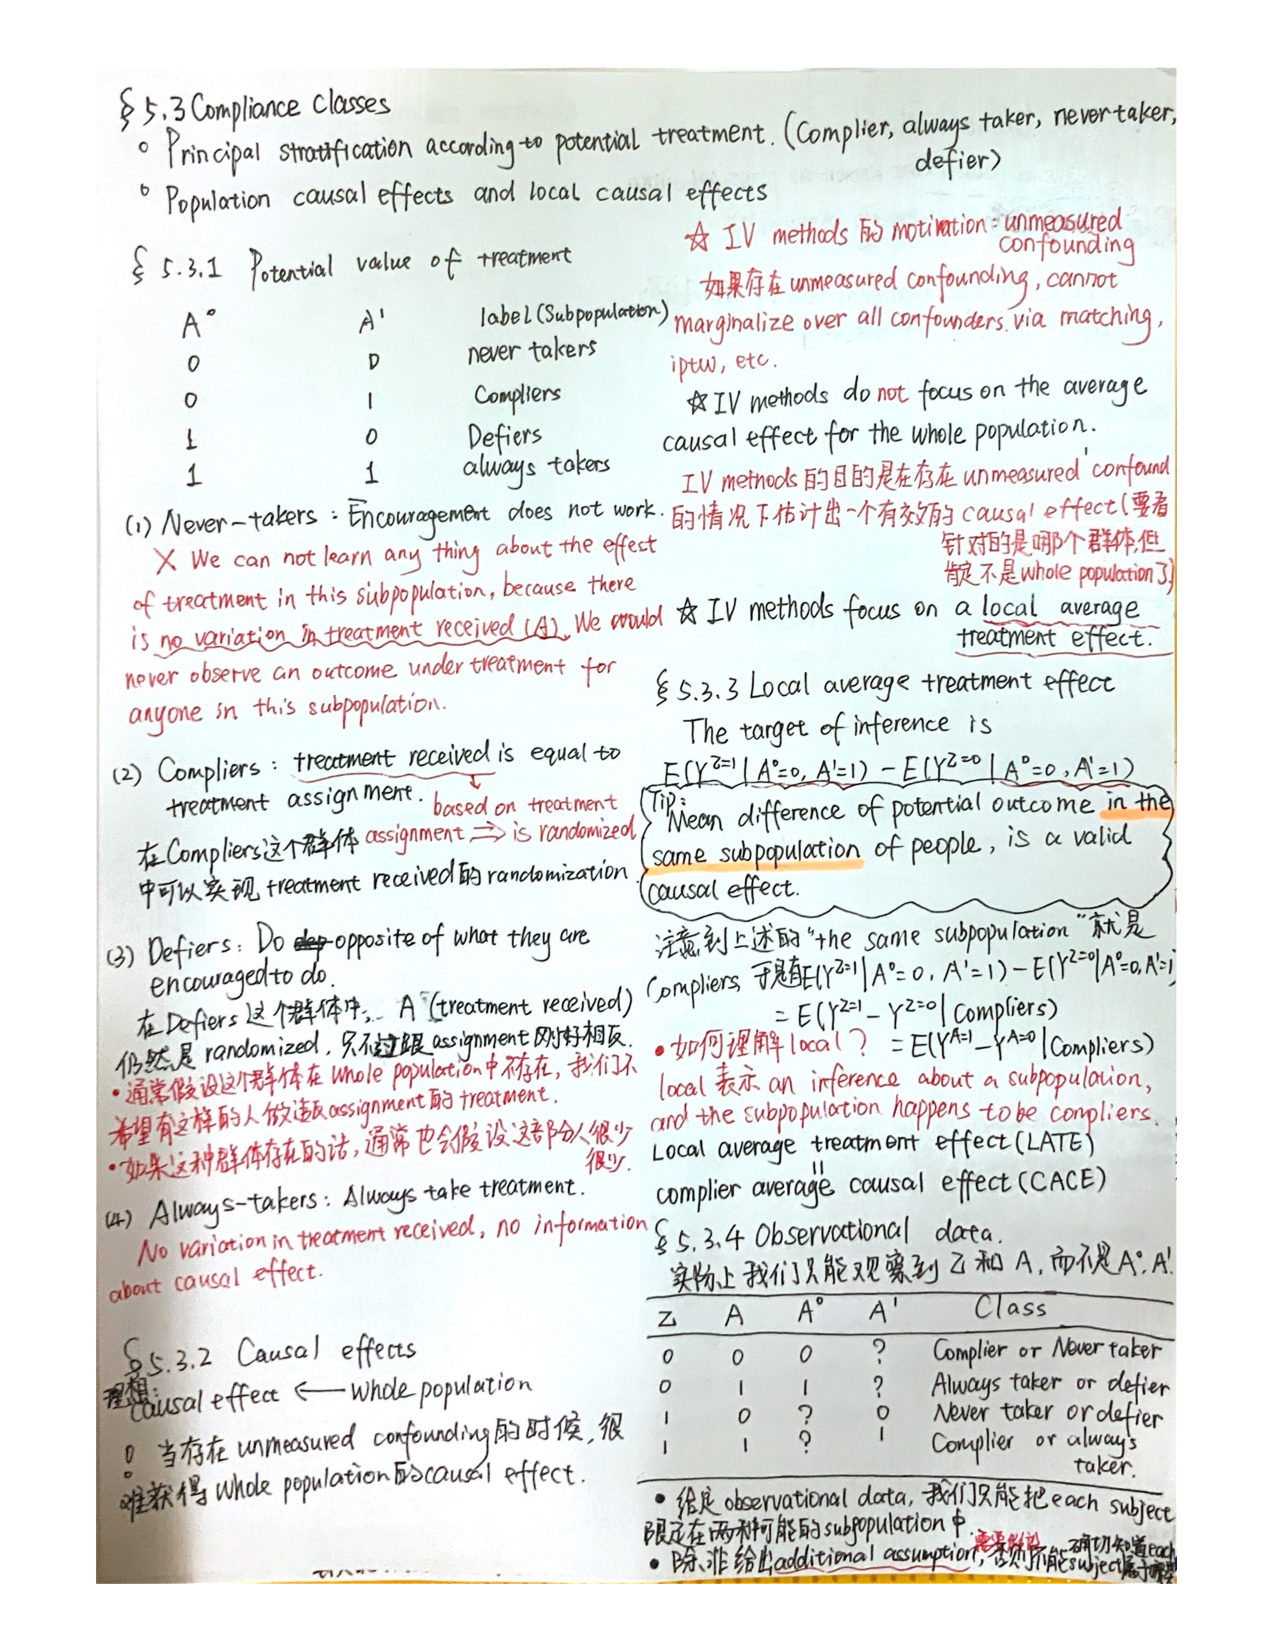
\includepdf[pages=-]{figure/5p2.pdf}
%
\includepdf[pages=-]{figure/5p3.pdf}
%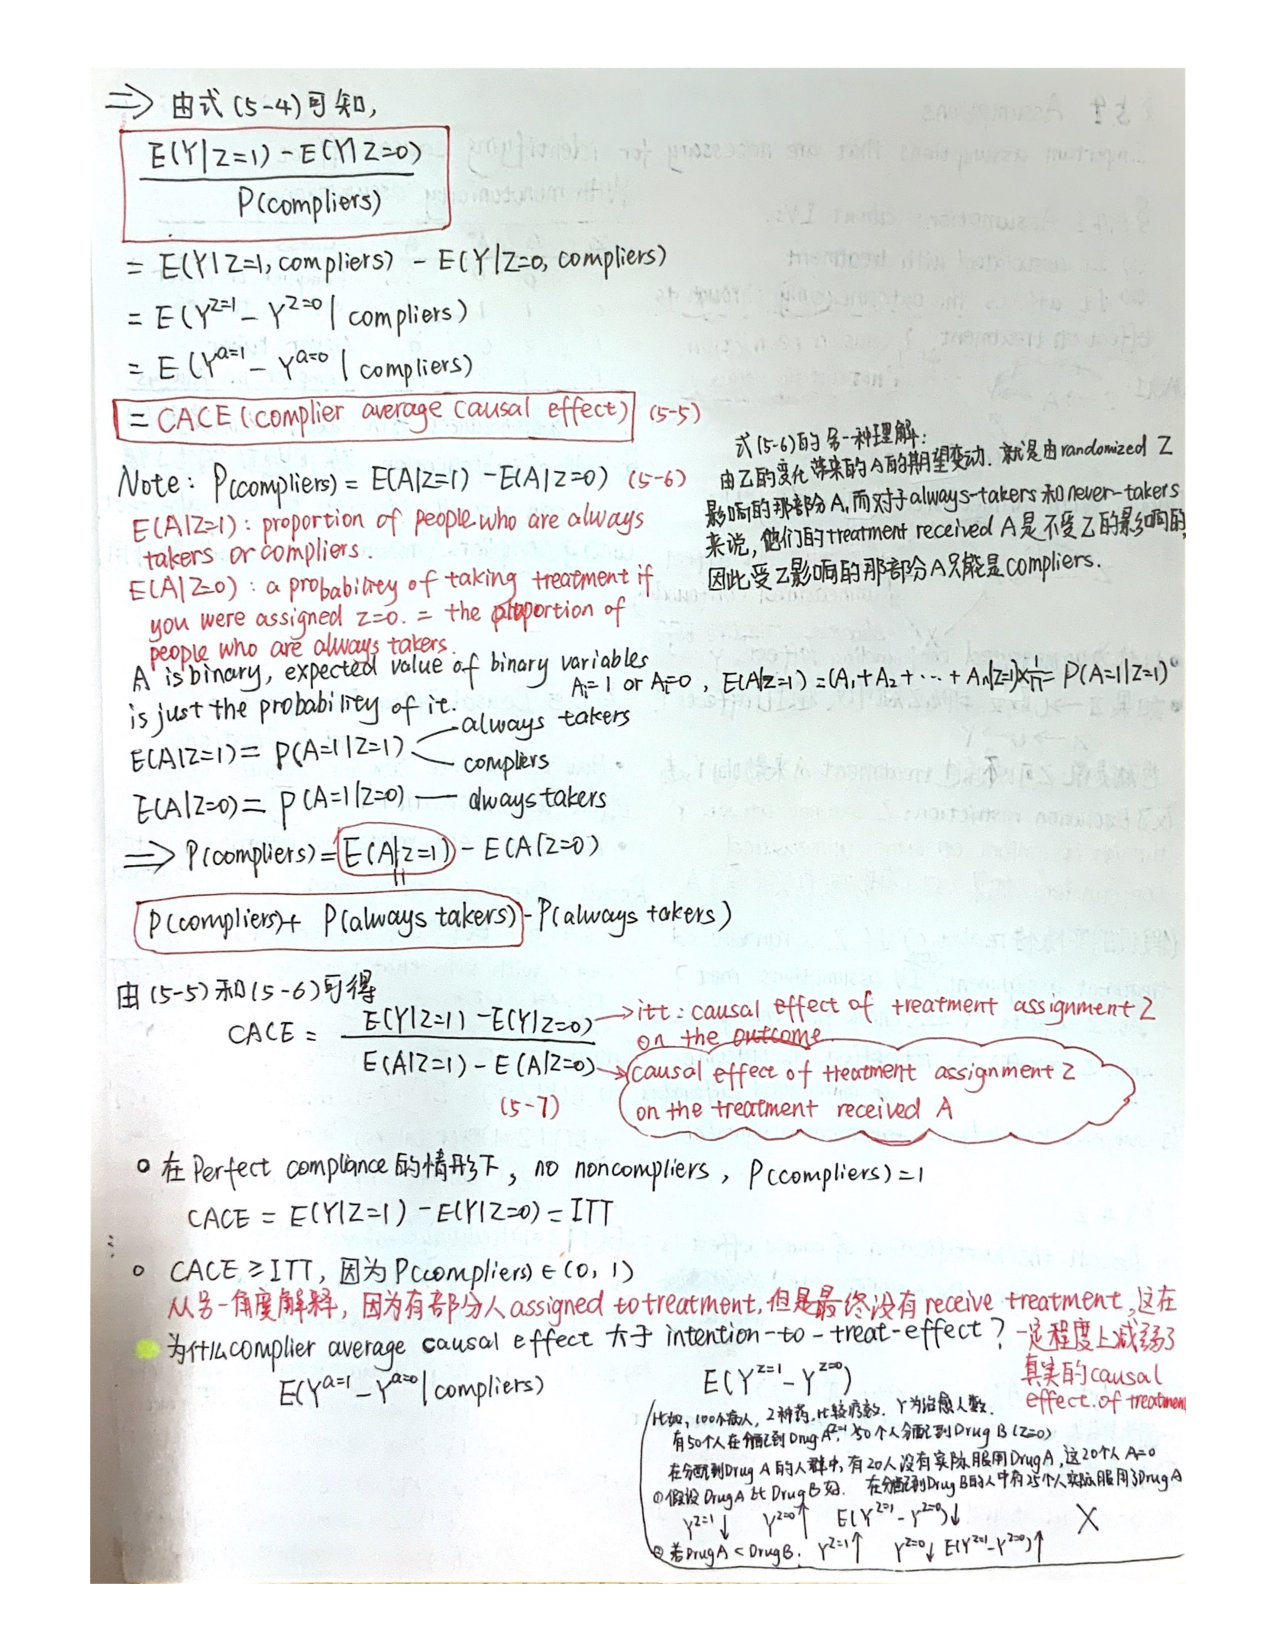
\includepdf[pages=-]{figure/5p4.pdf}